%%%
%
% $Autor: Wings $
% $Datum: 2021-05-14 $
% $Pfad: GitLab/MLEdgeComputer $
% $Dateiname: SensorHCSR04
% $Version: 4620 $
%
% !TeX spellcheck = de_DE/GB
% !TeX program = pdflatex
% !BIB program = biber/bibtex
% !TeX encoding = utf8
%
%%%

\chapter{Ultraschallsensor HC-SR04}


Introduction
\Mynote{cite books, applications, board}

\section{Domänenwissen}
Im folgenden Abschnitt wird der namensgebende Sensor für diese Arbeit näher betrachtet. Dazu zählen seine physikalischen Grundlagen, seine Funktionsweise und Anwendungsbeispiele aus Industrie und Medizin.

\section{Grundlagen zur Verwendung eines Ultraschallsensors}

\subsection{Grundlagen Schall}

Als Schall bezeichnet man die Ausbreitung von lokalen Druckschwankungen in einem elastischen Medium. Die Schallwelle breitet sich dabei longitudinal aus, die Auslenkung der Moleküle erfolgt also in Ausbreitungsrichtung \cite{Tippler:2024}.
Die Einteilung der Schallbereiche erfolgt auf Grundlage der Frequenz:

\begin{itemize}
    \item \textit{Infraschall:} bis 16 Hz,
    \item \textit{Hörbarer Schall:} von 16 Hz bis 20 kHz,
    \item \textit{Ultraschall:} von 20 kHz bis 1 GHz,
    \item \textit{Hyperschall:} über 1 GHz \cite{Hering:2023}.
\end{itemize}

\Mynote{Grafik fehlt}


\subsection{Schallgeschwindigkeit und Wellenlänge}\label{AbschnittVschall}

Die Geschwindigkeit, mit der sich Schall in Luft ausbreitet, ist von der Lufttemperatur $T$ und der Luftfeuchtigkeit $\varphi$ abhängig. Da die Luftfeuchtigkeit einen erheblich geringeren Einfluss auf den Wert hat 

\begin{equation}
    \Delta v_{Schall,\varphi}\approx1,2\:\dfrac{\text{m}}{\text{s}}; \:0<\varphi<1, \:T_{C}=20 \:\text{\textcelsius},
    \label{Vphi}
\end{equation}

\cite{Hering:2023} lässt sich die Schallgeschwindigkeit mit ausreichender Genauigkeit mit der Formel \ref{Vschall}

\begin{equation}
    v_{Schall}=\sqrt{\kappa R T}
    \label{Vschall}
\end{equation} 

und der Annahme $\varphi=0$ berechnen \cite{Tippler:2024}. 
Dabei ist $\kappa = 1{,}4$ der Adiabatenexponent von Luft, $R=287$ \(\dfrac{\text{J}}{\text{kg K}}\) die spezifische Gaskonstante von Luft und $T$ die absolute Temperatur in Kelvin \cite{Tippler:2024,Willems:2022}.
Für eine angenommene Temperatur von $T_{C} = 20\:\text{\textcelsius}$ ergibt sich damit eine Geschwindigkeit von $v_{Schall}=343,2\:\dfrac{\text{m}}{\text{s}}$.
In Abb. \ref{schallfunktion} ist die Schallgeschwindigkeit in Luft im Temperaturbereich von $T_{C} = -10 \:\text{\textcelsius \:bis} \:60 \:\text{\textcelsius}$ dargestellt.

\begin{figure}[h]
    \begin{center}
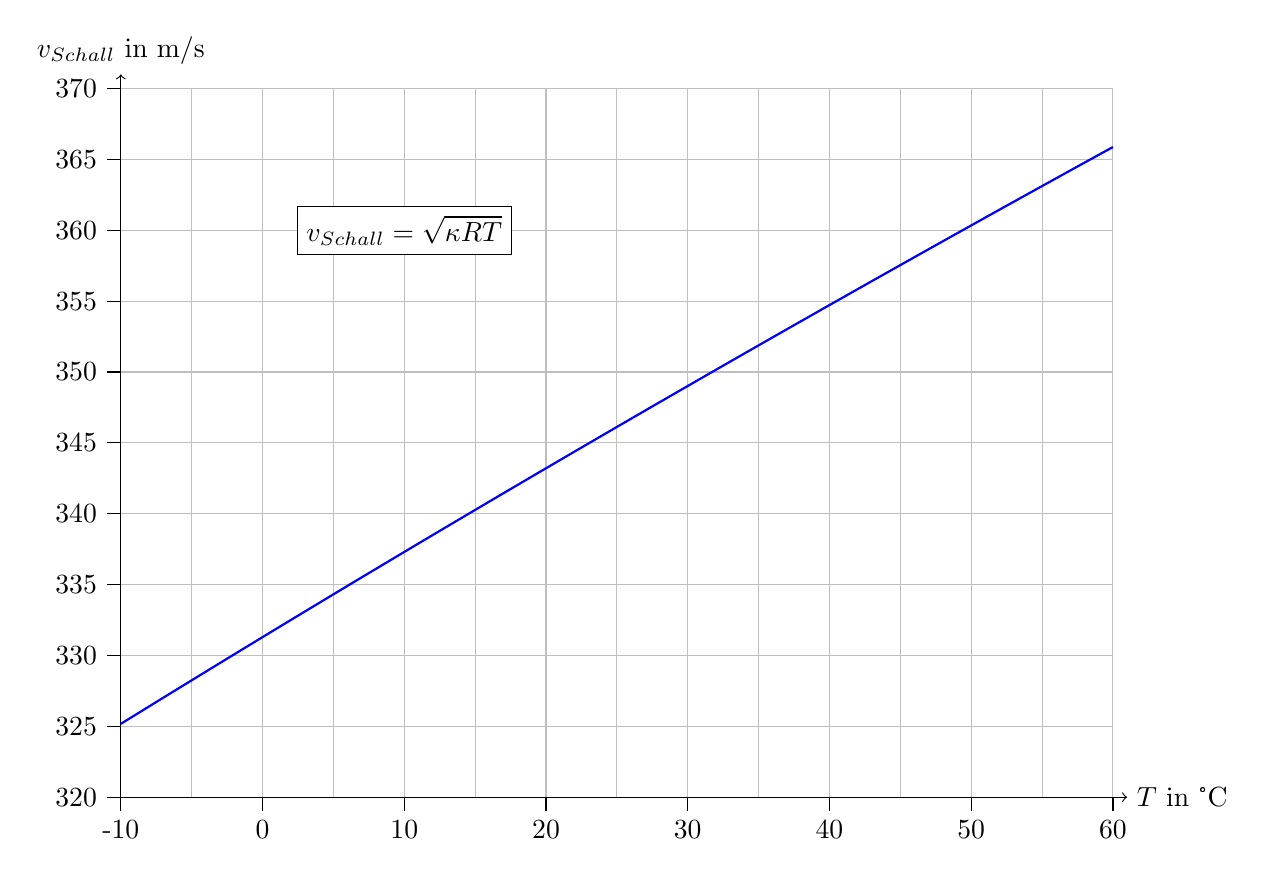
\begin{tikzpicture}
    \begin{scope}[scale=.9]
        %Gitter im Hintergrund
        \draw[lightgray] (-2,4) grid (12,14); 
        
        %Achsen
        \draw[thin, ->] (-2,4) -- (12.2,4) node[right] {$T$ in °C}; %x-Achse
        \draw[thin, ->] (-2,4) -- (-2,14.2) node[above] {$v_{Schall}$ in m/s}; %y-Achse
        %Beschriftung
        \foreach[count=\x] \a in {-10, 0, 10, 20, 30, 40, 50, 60} {
            \draw[thin] (2*\x-4,4) -- (2*\x-4,3.8) node [below] {\a};
        }%x-Achse
        \foreach[count=\x] \a in {320, 325, ..., 370} {
            \draw[thin] (-2,\x+3) -- (-2.2,\x+3) node [left] {\a};
        }%y-Achse
        
        %Funktion
        \draw[scale=2, thick, domain=26.316:33.316, variable=\T, blue] plot ({\T-27.316}, {sqrt(\T*40.18)-30});
        \node at(2,12) [rectangle,fill=white, draw] {$v_{Schall}=\sqrt{\kappa R T}$};
        
        %Vergleichsfunktion
        %\draw[gray] plot coordinates {(-2,5) (12,13.2)};
    \end{scope}
\end{tikzpicture}        \caption{Ausbreitungsgeschwindigkeit von Schall in Luft}
        \label{schallfunktion}
    \end{center}
\end{figure}

Über den Formelzusammenhang \ref{Wellenlaenge}

\begin{equation}
    v_{Schall}=\lambda f
    \label{Wellenlaenge}
\end{equation}

lässt sich bei gegebener Frequenz $f$ und mit der berechneten Schallgeschwindigkeit $v_{Schall}$ die Wellenlänge des Schalls berechnen \cite{Willems:2022}. Diese beträgt bei einer angenommenen Frequenz von $f=40 \:\text{kHz}$ und der in Abschnitt \ref{AbschnittVschall} berechneten Schallgeschwindigkeit $\lambda=8{,}58*10^{-3} \:\text{m}$.

\subsection{Absorption und Reflexion}

Absorption beschreibt die Abnahme der Intensität $I$ einer Schallwelle, während sie Weg durch das sie leitenden Medium zurücklegt. Sie ist vom Quadrat der Frequenz $f$ des Schalls und den Absorptionseigenschaften $a$ des Ausbreitungsmediums abhängig und lässt sich über die Formel \ref{Absorption}

\begin{equation}
    I(x)=I_0\times\exp(-\alpha x); \:\alpha=af^2
    \label{Absorption}
\end{equation}

berechnen \cite{Hering:2023,Hering:2021b}.
In Abbildung~\ref{DiagrammIntensitaet} ist die Abhängigkeit des Verhältnisses der Intensität $I$ zu $I_0$ von der Frequenz dargestellt. Die Wegstrecke von einem Meter und die Umgebungsbedingungen sind entsprechend konstant.

Für eine Frequenz von $f=40 \:\text{kHz}$ ergibt sich ein Verhältnis von 0,95.

\begin{figure}[h]
    \begin{center}
%Diagramm Intensität
%Abstandssensor\Entwicklerdokumentation\tikz
%tikz-Diagramm für die Abhängigkeit der Intensität von der Frequenz (qualitativ)
%Bestandteil der Entwicklerdokumentation "Abstandssensor" (Automatisierungstechnik SS24)

\begin{tikzpicture}
    \begin{scope}[scale=.85]	
        %Achsen
        \draw[thin, ->] (0,0) -- (10.2,0) node[right] {$f$ in KHz}; %x-Achse
        \draw[thin, ->] (0,0) -- (0,8.2) node[above] {$I/I_0$}; %y-Achse
        %Beschriftung
        \foreach[count=\x] \a in {0, 20, ..., 200} {
            \draw[thin] (\x-1,0) -- (\x-1,-0.2) node [below] {\a};
        }%x-Achse
        \foreach[count=\x] \a in {0.0001, 0.0010, 0.0100, 0.1000, 1.0000} {
            \draw[thin] (0,\x*2-2) -- (-0.2,\x*2-2) node [left] {\a};
        }%y-Achse
        
        %Funktion, qualitativ!
        \draw[thick, domain=0:10, variable=\x, blue] plot ({\x}, {-0.0741*\x^2+8});
    \end{scope}
\end{tikzpicture}
        \caption{Abnahme der Schallintensität in Abhängigkeit der Frequenz bei einem Meter, nach \cite{Hering:2023}}
        \label{DiagrammIntensitaet}
    \end{center}
\end{figure}

Trifft die Schallwelle auf die Grenzschicht zweier Medien mit verschiedenen Schallkennimpedanzen $Z_n$, wird sie zum Teil reflektiert und zum anderen Teil transmittiert. Der Reflexionsgrad ist bei großen Differenzen zwischen den Impedanzen $\left(Z_1 \ll Z_2 \:\text{oder} \:Z_1 \gg Z_2\right)$ der Medien besonders hoch. Sind die Impedanzen hingegen ähnlich $\left(Z_1 \approx Z_2\right)$ ist der Absorptionsgrad sehr hoch \cite{Hering:2021b}. 
Da viele Flüssigkeiten und feste Stoffe eine um den Faktor $10^4 \:\text{bis} \:10^5$ höhere Impedanz im Vergleich zu Luft vorweisen, ist der Reflexionsgrad in diesen Fällen $\gg 99\%$ \cite{Hering:2021b,Hering:2023}.

\subsection{Weg- und Abstandsmessung mit Ultraschall}

Um eine Entfernung oder einen Abstand eines Objekts zu dem Sensor zu ermitteln, wird der Sensor im sog. \textit{Tastbetrieb mit Echo-Laufzeit-Messung}, wie in Abb. \ref{TastbetriebELM} zu sehen, verwendet. Dabei sendet der Sensor zunächst ein Schallpuls in Richtung des zu messenden Objekts aus (Lautsprecher), welche zum Teil von diesem reflektiert wird und somit zurück zum Sensor gelangt (Echo). Dieses Echo kann der Sensor detektieren (Mikrofon) und über die gemessene Laufzeit des Echos sowie die Schallgeschwindigkeit im dem den Sensor umgebenden Medium die Distanz berechnen \cite{Hering:2023}.

\begin{figure}[h]
    \begin{center}
%Funktionsweise
%Abstandssensor\Entwicklerdokumentation\tikz
%tikz-Diagramm zur Funktionsweise eines Ultraschallsensors (qualitativ)
%Bestandteil der Entwicklerdokumentation "Abstandssensor" (Automatisierungstechnik SS24)

\begin{tikzpicture}
    %Achsen
    \draw[thin, ->] (0,0) -- (10.2,0) node[right] {$t$}; %x-Achse
    \draw[thin, ->] (0,0) -- (0,4.2) node[above] {$U$}; %y-Achse
    
    %Funktion, qualitativ!
    \draw[thick, blue] plot [smooth] coordinates{(1,0) (2,3) (4,3.5) (4.5,1) (5,0.1) (6,0)};
    \draw[thick, blue] plot [smooth] coordinates{(8,0) (8.3,0.1) (9,0.8) (9.7,0.1) (10,0)};
    
    %Beschriftung
    \node at (1,0) [anchor=south east] {$t_0$};
    \node at (8,0) [anchor=south east] {$t_1$};
    \draw[dotted] (4.5,1) -- (5,2) node[anchor=south west]{Sendeimpuls}; 
    \draw[dotted] (9,0.8) -- (9.5,2) node[anchor=south]{Echo}; 
    \draw (1,0) -- (1,-2.2);
    \draw (8,0) -- (8,-2.2);
    \draw[<->] (1,-2) -- (4.5,-2) node[anchor=south]{Echolaufzeit} -- (8,-2);
    \draw (4,0) -- (4,-1.2); 
    \draw (6,0) -- (6,-1.2); 
    \draw[<->] (1,-1) -- (2.5,-1) node[anchor=south]{$\delta t$} -- (4,-1);
    \draw[<->] (4,-1) -- (5,-1) node[anchor=south]{\tiny{Ausschwingzeit}} -- (6,-1);
\end{tikzpicture}
        \caption{Spannungsverlauf Schallwandler bei einer Echo-Laufzeit-Messung, nach \cite{Hering:2023}}
        \label{TastbetriebELM}
    \end{center}
\end{figure}

In der Anwendung einköpfiger Sensoren ist für die Messung sehr kleiner Distanzen auf die Ausschwingzeit des Wandlers sowie die Umschaltzeit vom Lautsprecher- in den Mikrofonbetrieb zu achten, da in dieser Zeit kein Echosignal aufgenommen werden kann. Bei zweiköpfigen Systemen, also je einem dedizierten Lautsprecher und Mikrofon, sind die Öffnungswinkel der Schallkeulen in Verbindung mit dem radialen Abstand maßgeblich für die minimale Distanz.  

Bei großen Distanzen sind sowohl die Genauigkeit der Ausrichtung des Sensors $\left(\text{bei kleinen Öffnungswinkeln der Schallkeulen}\right)$ als auch die Absorption der Schallintensität in dem Ausbreitungsmedium relevant \cite{Hering:2023}. 

Ebenfalls störend auswirken können sich die Geometrie des zu messenden Objektes $\left(\text{z. B. bei stark konkaven oder konvexen Oberflächen}\right)$, absorbierendes/diffus reflektierendes Material $\left(\text{Filz, Watte, Schaumstoff}\right)$ oder Umwelteinflüsse orthogonal zur Messrichtung wirkender Wind. Verunreinigungen wie Staub und Rauch oder leichter Niederschlag in Form von Regen und Schnee beeinträchtigen die Messung hingegen nicht \cite{Hering:2023}.

\subsection{Anwendungen}

Ultraschallsensoren haben in der Praxis ein breites Einsatzgebiet \cite{Hering:2023}. Basierend auf dem Ausbreitungsmedium lassen sie sich in drei Kategorien einteilen.

Die erste Kategorie wird dem Luftschall zugeschrieben. Typische Anwendungsbeispiele sind Füllstandsensoren, Durchmessererfassung für Auf- und Abwickelsteuerung oder Kollisionsschutz/Objekterkennung \cite{Hering:2023}.

Bei Sensoren der zweiten Kategorie breitet sich der Schall über Flüssigkeiten aus, wodurch diese vor allem im maritimen Bereich anzutreffen sind. Als Beispiele sind Sonarsysteme zum Orten von Unterseebooten oder Fischschwärmen und das Echolot zur Kartografie des Meeresbodens zu nennen \cite{Hering:2021b}.

Die dritte Kategorie umfasst Körperschallsensoren. Viel verwendetes Beispiel in der Industrie sind Sensoren zur zerstörungsfreien Materialprüfung. In der Medizin ist die bildgebende Ultraschalldiagnostik ein wichtiges Werkzeug zur Überprüfung von Organen oder Föten \cite{Hering:2021b}.


\subsection{Herausforderungen}

Dadurch, dass die Schallgeschwindigkeit von der Umgebungstemperatur abhängig ist, muss diese für die Berechnung der Distanz mit einbezogen werden, wenn der Sensor in einem größeren Temperaturbereich eingesetzt werden soll. In Abbildung~\ref{schallfunktion} ist zu erkennen, dass die Differenz der Geschwindigkeit in dem Temperaturbereich, in dem alle Komponenten des Sensors betrieben werden könnten $\left(-10 \:\text{\textcelsius}\leq T_{C}\leq55 \:\text{\textcelsius}\right)$, etwa $38 \:\dfrac{\text{m}}{\text{s}}$ beträgt. Dies entspricht, ausgehend von dem Standardwert für die Schallgeschwindigkeit $v_{Schall,20}=343,2\:\dfrac{\text{m}}{\text{s}}$, einer Streuung von $-5,2\% \:\text{und} \:+5,8\%$. Hinzu kommt die Unsicherheit aufgrund der Luftfeuchtigkeit. Hier liegt die Streuung, bezogen auf die Schallgeschwindigkeiten bei $\varphi=0$, in einem Bereich zwischen $+0,37\% \:\text{für} \:T_{C}=-10\:\text{\textcelsius} \:\text{und} \:+0,33\% \:\text{für} \:T_{C}=55 \:\text{\textcelsius}$.

Physikalische Effekte wie die Absorption, welche unter Laborbedingungen maßgeblich die Reichweite des Sensors einschränkt, oder einen schlechten Reflexionsgrad bestimmter Materialien, schränken das System in seiner Vielseitigkeit ein. Selbiges gilt für Attribute des Sensors wie die Ausschwingzeit des Schallwandlers oder die geometrische Anordnung der Schallkeulen bei zweiköpfigen Systemen.
Auch die genannten Umwelteinflüsse können dafür sorgen, dass eine Messung fehlschlägt oder ein falsche Ergebnis liefert.

\subsection{Lösungsansätze}

Um große mögliche Messfehler aufgrund einer fest hinterlegten Schallgeschwindigkeit zu vermeiden, soll die Temperatur von dem internen Temperatursensor des Arduino Nano 33 BLE Sense Lite bei einer Abstandsmessung erfasst und auf dessen Grundlage die Schallgeschwindigkeit berechnet werden. Da der Sensor jedoch auf der Platine ist, diese sich bei Benutzung selbst erwärmt und zusätzlich in einem Gehäuse verbaut ist, dessen Material gute wärmeisolierende Eigenschaften hat, ist die von ihm gemessene Temperatur zeitabhängig. Daraus folgt, dass seine Messwerte nicht für die Berechnung der Schallgeschwindigkeit verwendet werden können.
Die Verwendung eines zusätzlichen Temperatursensors wäre eine mögliche Lösung. Daher wird, um eine zu große Abweichung des angezeigten Messwertes zu verhindern, der für den Sensor zugelassene Temperaturbereich eingeschränkt. Ein möglicher Temperaturbereich ist zwischen $17 \:\text{\textcelsius \:und} \:23 \:\text{\textcelsius}$. In diesem Bereich liegt die Abweichung der Schallgeschwindigkeit bei unter $0,5\%$. Ob diese Genauigkeit ausreichend ist, ist von der Anwendung abhängig.


\section{Ultraschall Abstandsensor}

Der Ultraschallabstandssensor in Abbildung~\ref{Ultraschall Abstandssensor} vom Hersteller JOY-it enthält den Sensor HC-SR04. Er ist als zweiköpfiger Sensor ausgeführt, wodurch er über je einen Lautsprecher und ein Mikrofon verfügt.

 und ist  zur Erfassung von Abständen in einem Bereich von 3 bis 400 cm spezifiziert. Dafür nutzt er eine Schallfrequenz von 40 kHz. Er ist als zweiköpfiger Sensor ausgeführt, wodurch er über je einen Lautsprecher und ein Mikrofon verfügt.  Die Abmessungen des Sensors betragen in der Breite 43 mm, in der Höhe 15 mm und in der Tiefe 20 mm. Die Auflösung des Sensors beträgt $\pm 1$ mm. Angeschlossen wird der Abstandssensor über den \ac{vcc}-Pin, Trig/\ac{scl}-Pin, Echo/\ac{sda}-Pin und dem \ac{gnd}-Pin. Der Sensor kann über die drei Schnittstellen \ac{gpio}, \ac{uart} und \ac{i2c} verbunden werden \cite{Simac:2017}. 

    \begin{center}
        \includegraphics[width=3in]{Sensor/HCSR04/HCSR04}
        \captionof{figure}{Ultraschallabstandssensor der Marke JOY-IT\cite{Simac:2017}}
        \label{Ultraschall Abstandssensor}
    \end{center}


\section{Specification}

 Der Sensor HC-SR04 ist  zur Erfassung von Abständen in einem Bereich von 3 bis 400 cm mit einer Auflösung von $\pm 1$mm spezifiziert. Dafür nutzt er eine Schallfrequenz von 40 kHz.   Die Abmessungen des Sensors betragen in der Breite 43 mm, in der Höhe 15 mm und in der Tiefe 20 mm. 
 
 Angeschlossen wird der Abstandssensor über den \ac{scl}-Pin für das Triggersignal, den \ac{sda}-Pin fürs Echo, den \ac{vcc}-Pin zur Stromversorgung und dem \ac{gnd}-Pin. 
 
 Der Sensor kann über die drei Schnittstellen \ac{gpio}, \ac{uart} und \ac{i2c} verbunden werden \cite{Simac:2017}. 


Bei den folgenden Beispielprogrammen wird der Arduino Nano 33 BLE Sense verwendet. In den Beispielen werden die Pins D6 und D9 für die Datenübertragung verwendet. In der Tabelle~\ref{PinBelegungUltraschall}  ist dies für die Grove-Schnittstelle festgehalten.

    \begin{center}
        \captionof{table}{Pinbelegung für den Ultraschallabstandssensor \cite{Simac:2017}}
        \begin{tabular}{c|c}
            Arduino Pin & Ultraschall Abstandssensor\\ \hline
            D9 & Trig\\
            D6 & Echo\\
            3V3 & \acs{vcc}\\
            \acs{gnd} & \acs{gnd}\\
        \end{tabular}
        \label{PinBelegungUltraschall}
    \end{center}



\section{Bibliothek}

\subsection{Description}


\subsection{Installation}

\subsection{Functions}

\subsection{Example - Manual}

\subsection{Example}

\subsection{Example - Code}

\subsection{Example - Files}



\section{Calibration}

\section{Kalibrierung}
Der Ultraschallabstandssensor wird für die Verwendung bei der Temperatur von 20 °C ausgelegt. Die  berechnete Schallgeschwindigkeit $v_{Schall}=343,2\:\dfrac{\text{m}}{\text{s}}$ bei 20 °C wird für die Umrechnung der Schalldauer in die Distanz zur Reflexionsfläche verwendet.

\Mynote{cite method}


\section{Simple Code}

\section{Einfacher Bespiel zur Verwednung des Ultraschallabstandsensors}

Mit dem Sketch \FILE{TestHCSR04 UltraschallsensorTest.ino} wird die Funktionalität des Ultraschallsensors getestet.

\begin{code}
    \pythonexternal[language=c++]{../../Code/Arduino/UltraSonicHCSR04/TestHCSR04.ino}
\end{code}


\subsection{Durchführung}

Für den Test werden die folgenden Hardware-Komponenten benötigt:

\begin{itemize}
    \item Arduino Nano 33 BLE Sense Lite
    \item Tiny Machine Learning Shield
    \item USB-A auf USB-Mikro Verbindungskabel
    \item Grove Jumper zu Grove 4 Pin Kabel
    \item Ultraschallsensor
\end{itemize}

Die Hardware-Komponenten werden verbunden und anschließend der  Arduino Nano 33 BLE Sense Lite mit einem Computer verbunden. Dann wird der Sketch \FILE{TestHCSR04.ino} auf den Arduino Nano 33 BLE Sense Lite geladen und der serielle Monitor in der Arduino \acs{ide} geöffnet. Ein Gegenstand wird ungefähr 20 cm orthogonal vor den Ultraschallsensor gehalten.

\subsection{Ergebnisse}

Der gemessene Abstand wird in Abbildung~\ref{BildUltraschallsensorTest} dargestellt und liegt in dem erwarteten Bereich. 

    \begin{center}
        \includegraphics[width=\textwidth]{Sensor/HCSR04/HCSR04Test}
        \captionof{figure}{Testoutput des Ultraschallsensors}
        \label{BildUltraschallsensorTest}
    \end{center}

\section{Simple Application}



\section{Tests}

\subsection{Simple Function Test}

\subsection{Test all Functions}

\section{Simple Application}


\section{Further Readings}


